% Chapter Template

\chapter{Results} % Main chapter title

\label{Chapter3} % Change X to a consecutive number; for referencing this chapter elsewhere, use \ref{ChapterX}

\lhead{Section 3. \emph{Results}} % Change X to a consecutive number; this is for the header on each page - perhaps a shortened title

%----------------------------------------------------------------------------------------
%	SECTION 1
%----------------------------------------------------------------------------------------

\section{Image Denoising}
\subsection{PSNR results in image denoising}

In order to assess the performance of various filter banks in image denoising, three images named Lena, Boat and Barbara respectively were chosen as the original image. Moreover, five different filter banks including two Daubechies filters and three tight framelet filters. In the following analysis, the ``Haar'' wavelet filter is referred as `db1' and the Daubechies 4-tap filter is referred as `db2'. Also, `tf1',`tf2' and `tf3' are representing three different kinds of tight framelet wavelet filters.
\begin{itemize}
    \item Orthogonal Filter Bank `db1' 
    \begin{itemize}
        \item $h_0 = \{\frac{1}{2},\frac{1}{2}\}$ \qquad $h_1 = \{-\frac{1}{2},\frac{1}{2}\}$
        \item $g_0 = \{\frac{1}{2},\frac{1}{2}\}$ \qquad $g_1 = \{-\frac{1}{2},\frac{1}{2}\}$

    \end{itemize}

    \item Orthogonal Filter Bank `db2' 
    \begin{itemize}
        \item $h_0 = \{\frac{1-\sqrt3}{8},\frac{-3+\sqrt3}{8},\frac{3+\sqrt3}{8},\frac{-1-\sqrt3}{8}\}$ \qquad $h_1 = \{\frac{1+\sqrt3}{8},\frac{3+\sqrt3}{8},\frac{3-\sqrt3}{8},\frac{1-\sqrt3}{8}\}$
        \item $g_0 = \{\frac{1-\sqrt3}{8},\frac{-3+\sqrt3}{8},\frac{3+\sqrt3}{8},\frac{-1-\sqrt3}{8}\}$ \qquad $g_1 = \{\frac{1+\sqrt3}{8},\frac{3+\sqrt3}{8},\frac{3-\sqrt3}{8},\frac{1-\sqrt3}{8}\}$
    \end{itemize}
    \item Tight Framelet Filter Bank `tf1' 
    \begin{itemize}
        \item $h_0 = \{\frac{1}{4},\frac{1}{2},\frac{1}{4}\}$ \qquad $h_1 = \{-\frac{\sqrt2}{4},0,\frac{\sqrt2}{4}\}$ \qquad $h_2 = \{-\frac{1}{4},\frac{1}{2},-\frac{1}{4}\}$
        \item $g_0 = \{\frac{1}{4},\frac{1}{2},\frac{1}{4}\}$ \qquad $g_1 = \{-\frac{\sqrt2}{4},0,\frac{\sqrt2}{4}\}$ \qquad $g_2 = \{-\frac{1}{4},\frac{1}{2},-\frac{1}{4}\}$
    \end{itemize}

    \item Tight Framelet Filter Bank `tf2' 
    \begin{itemize}

        \item $h_0 = \{\frac{5}{1024},0,-\frac{63}{1024},\frac{75}{1024},\frac{495}{1024},\frac{495}{1024},\frac{75}{1024},-\frac{63}{1024},0,\frac{5}{1024}\}$ \\ 
        $h_1 = \{0,0,-\frac{3\sqrt{15}}{512},0,\frac{22\sqrt{15}}{512},-\frac{45\sqrt{15}}{512},\frac{45\sqrt{15}}{512},-\frac{22\sqrt{15}}{512},0,\frac{3\sqrt{15}}{512}\}$ \\
        $h_2 = \{\frac{5}{1024},0,-\frac{117}{1024},\frac{75}{1024},\frac{315}{1024},-\frac{315}{1024},-\frac{75}{1024},\frac{117}{1024},0,-\frac{5}{1024}\}$ \\ 
        \item $g_0 = \{\frac{5}{1024},0,-\frac{63}{1024},\frac{75}{1024},\frac{495}{1024},\frac{495}{1024},\frac{75}{1024},-\frac{63}{1024},0,\frac{5}{1024}\}$ \\ 
        $g_1 = \{0,0,-\frac{3\sqrt{15}}{512},0,\frac{22\sqrt{15}}{512},-\frac{45\sqrt{15}}{512},\frac{45\sqrt{15}}{512},-\frac{22\sqrt{15}}{512},0,\frac{3\sqrt{15}}{512}\}$ \\
        $g_2 = \{\frac{5}{1024},0,-\frac{117}{1024},\frac{75}{1024},\frac{315}{1024},-\frac{315}{1024},-\frac{75}{1024},\frac{117}{1024},0,-\frac{5}{1024}\}$ \\ 
    \end{itemize}
    \item Tight Framelet Filter Bank `tf3' 
    \begin{itemize}
        \item $h_0 = \{\frac{63}{5120},0,-\frac{-429}{5120},0,\frac{1309}{5120},\frac{1617}{5120},\frac{1617}{5120},\frac{1309}{5120},0,-\frac{429}{5120},0,\frac{63}{5120}\}$ \\ 
        $h_1 = \{0,0,\frac{3\sqrt{231}}{2560},0,\frac{10\sqrt{231}}{2560},0,-\frac{77\sqrt{231}}{2560},\frac{77\sqrt{231}}{2560},0,-\frac{10\sqrt{231}}{2560},0,-\frac{3\sqrt{231}}{2560}\}$ \\
        $h_2 = \{\frac{63}{5120},0,-\frac{495}{5120},0,\frac{385}{5120},\frac{1617}{5120},-\frac{1617}{5120},-\frac{385}{5120},0,-\frac{495}{5120},0,-\frac{63}{5120}\}$ \\ 
        \item $g_0 = \{\frac{63}{5120},0,-\frac{-429}{5120},0,\frac{1309}{5120},\frac{1617}{5120},\frac{1617}{5120},\frac{1309}{5120},0,-\frac{429}{5120},0,\frac{63}{5120}\}$ \\ 
        $g_1 = \{0,0,\frac{3\sqrt{231}}{2560},0,\frac{10\sqrt{231}}{2560},0,-\frac{77\sqrt{231}}{2560},\frac{77\sqrt{231}}{2560},0,-\frac{10\sqrt{231}}{2560},0,-\frac{3\sqrt{231}}{2560}\}$ \\
        $g_2 = \{\frac{63}{5120},0,-\frac{495}{5120},0,\frac{385}{5120},\frac{1617}{5120},-\frac{1617}{5120},-\frac{385}{5120},0,-\frac{495}{5120},0,-\frac{63}{5120}\}$ \\ 

    \end{itemize}
\end{itemize}

In table 3.1, 3.2 and 3.3, the columns refer to five filter banks respectively and the rows represent cases in different noise levels. In the experiment, several possible combination of different coefficients (e.g. Decomposition Levels, Threshold values...) were tried in order to obtain the near optimal performance of a method as much as possible. Moreover, both soft thresholding and hard thresholding schemes were implemented and the results can be easily compared in the cells. Finally, the following three tables present the nearly optimal PSNR values for different methods and various noise levels. The result of the method with the best performance is highlighted in bold font for each test set.\\

\begin{algorithm} 
\caption{Obtaining the optimum denoising result}  
\label{alg:4}  
\begin{algorithmic}
\REQUIRE ~~\\ %算法的输入参数:Input  
A choices set L for possible levels (e.g. L= [3:7])
A choices set TV for possible threshold values (e.g. TV = [50:25:300])
\ENSURE ~~\\ %算法的输出:Output  
The optimum $PSNR_{opt}$ and the optimum Indices $i_{opt},j_{opt}$
\STATE let $PSNR_{opt} = 0$
\STATE let $i_{opt} , j_{opt} =0$
\FOR {i = 1: length(L)}
\STATE $l = L(i)$
\FOR {j = 1: length(TV)}
\STATE $th = TV(j)$
\STATE Using denoising algorithm to compute the PSNR with Decomposition levels = l and threshold value = th
\IF {$PSNR > PSNR_{opt}$}
\STATE $PSNR_{opt} = PSNR, \; i_{opt} = i,\; j_{opt} = j$ 
\ENDIF
\ENDFOR
\ENDFOR

\end{algorithmic}  
\end{algorithm}  
\vfill
% Please remember to add \use{multirow} to your document preamble in order to suppor multirow cells
\begin{table}[h]
\resizebox{1\textwidth}{!}{
\begin{tabular}{|c|l|l|l|l|l|l|l|l|l|l|}
\hline
\multirow{2}{*}{Lena} & \multicolumn{2}{|l}{db1} & \multicolumn{2}{|l}{db2} & \multicolumn{2}{|l}{tf1} & \multicolumn{2}{|l}{tf2} & \multicolumn{2}{|l|}{tf3} \\ \cline{2-11} 
 & hard & soft & hard & soft & hard & soft & hard & soft & hard & soft \\ \hline
 $\sigma=5$ & \bf{29.56} & 26.61 & 33.01 & 19.94 & 29.07 & 25.59 & 30.04 & 26.38 & 28.69 & 25.35 \\ \hline
 $\sigma=5$ & 29.43 & 26.61 & \bf{31.02} & 19.81 & 29.04 & 25.58 & 29.98 & 26.35 & 28.67 & 25.34 \\ \hline
 $\sigma=15$ & 28.91 & 26.65 & 28.76 & 19.63 &\bf{29.02} & 25.58 & 29.83 & 26.32 & 28.66 & 25.34 \\ \hline
 $\sigma=20$ & 27.04 & 26.65 & 26.06 & 19.36 & 28.92 & 25.56 & \bf{29.60} & 26.25 & 28.49 & 25.31 \\ \hline
 $\sigma=30$ & 26.00 & 25.98 & 21.67 & 18.69 & 27.80 & 25.51 & \bf{28.51} & 26.12 & 26.69 & 25.25 \\ \hline
 $\sigma=50$ & 23.85 & 23.45 & 17.51 & 16.68 & 25.54 & 24.60 & \bf{25.94} & 25.30 & 24.74 & 24.11 \\ \hline
 $\sigma=100$ & 18.43 & 19.98 & 11.60 & 12.47 & 21.78 & 20.59 & \bf{22.05} & 21.22 & 21.80 & 20.50 \\ \hline
 \end{tabular}}
\caption{Lena Denoising}
 \end{table}

% Boat
\begin{table}[h]
\resizebox{1\textwidth}{!}{
\begin{tabular}{|l|l|l|l|l|l|l|l|l|l|l|}
\hline
\multicolumn{1}{|c}{\multirow{2}{*}{Boat}} & \multicolumn{2}{|l}{db1} & \multicolumn{2}{|l}{db2} & \multicolumn{2}{|l}{tf1} & \multicolumn{2}{|l}{tf2} & \multicolumn{2}{|l|}{tf3} \\ \cline{2-11} 
\multicolumn{1}{|c|}{} & hard & soft & hard & soft & hard & soft & hard & soft & hard & soft \\ \hline
$\sigma=5$ & 28.28 & 25.49 & \bf{30.07} & 19.80 & 27.23 & 24.09 & 27.98 & 24.81 & 26.83 & 23.88 \\ \hline
$\sigma=10$ & 28.12 & 25.49 & \bf{28.88} & 19.70 & 27.23 & 24.09 & 27.91 & 24.79 & 26.83 & 23.87 \\ \hline
$\sigma=15$ & 27.68 & 25.52 & 27.33 & 19.54 & 27.20 & 24.08 & \bf{27.84} & 24.78 & 26.78 & 23.87 \\ \hline
$\sigma=20$ & 26.18 & 25.52 & 25.26 & 19.31 & 27.16 & 24.09 & \bf{27.67} & 24.76 & 26.69 & 23.87 \\ \hline
$\sigma=30$ & 24.81 & 25.02 & 22.09 & 18.67 & 26.29 & 24.03 & \bf{26.66} & 24.65 & 25.42 & 23.83 \\ \hline
$\sigma=50$ & 22.65 & 22.58 & 17.65 & 16.64 & 23.90 & 23.37 & \bf{24.28} & 23.86 & 23.29 & 22.97 \\ \hline
$\sigma=100$ & 17.99 & 19.57 & 11.71 & 12.34 & \bf{20.84} & 19.76 & 21.09 & 20.53 & \bf{20.84} & 19.63 \\ \hline
\end{tabular}}
\caption{Boat Denoising}
\end{table}


%Barbara
\begin{table}[h]
\resizebox{1\textwidth}{!}{
\begin{tabular}{|l|l|l|l|l|l|l|l|l|l|l|}
\hline
\multicolumn{1}{|c}{\multirow{2}{*}{Barbara}} & \multicolumn{2}{|l}{db1} & \multicolumn{2}{|l}{db2} & \multicolumn{2}{|l}{tf1} & \multicolumn{2}{|l}{tf2} & \multicolumn{2}{|l|}{tf3} \\ \cline{2-11} 
\multicolumn{1}{|c|}{} & hard & soft & hard & soft & hard & soft & hard & soft & hard & soft \\ \hline
$\sigma=5$ & 26.62 & 24.06 & \bf{29.65} & 19.50 & 25.32 & 22.96 & 26.65 & 23.67 & 25.48 & 22.98 \\ \hline
$\sigma=10$ & 26.48 & 24.10 & \bf{28.41} & 19.40 & 25.35 & 22.97 & 26.65 & 23.66 & 25.50 & 22.99 \\ \hline
$\sigma=15$ & 26.10 & 24.14 & \bf{26.82} & 19.25 & 25.41 & 22.98 & 26.58 & 23.66 & 25.50 & 23.00 \\ \hline
$\sigma=20$ & 24.92 & 24.17 & 24.84 & 19.04 & 25.41 & 23.00 & \bf{26.48} & 23.66 & 25.46 & 23.02 \\ \hline
$\sigma=30$ & 23.24 & 23.92 & 20.94 & 18.46 & 24.98 & 23.05 & \bf{25.81} & 23.65 & 24.52 & 23.05 \\ \hline
$\sigma=50$ & 21.72 & 21.76 & 17.14 & 16.61 & 22.87 & 22.72 & \bf{23.27} & 23.22 & 22.59 & 22.55 \\ \hline
$\sigma=100$ & 17.68 & 19.14 & 11.33 & 12.56 & 20.29 & 19.91 & \bf{20.58} & 20.18 & 20.39 & 19.89 \\ \hline
\end{tabular}}
\caption{Barbara Denoising}
\end{table}



%-----------------------------------
%	SUBSECTION 2
%-----------------------------------

\subsection{Performance analysis}
In terms of thresholding schemes, the choice of hard thresholding gives a better performance evaluated by PSNR. In contrast, soft thresholding generates a poorer result in almost every test case. As the optimum data highlighted in bold illustrates, the filter banks `db2' and `tf1' have demonstrated a great advantage in image denoising over the other filter banks. To be specific, the data indicates that the tight framelet filter banks are preferable in the circumstances with higher noise levels and `db2' is preferable in the cases with lower noise levels. Figure 3.1 shows the difference between methods using orthogonal filter bank `db2' and tight framelet filter bank `tf2' in the performance of denoising with $\sigma = 30$. Moreover, the second column gives the zoom in graphs in order to show the details.
\begin{figure}[H]
\begin{minipage}[t]{0.55\textwidth}
\centering
\resizebox{5cm}{5cm}{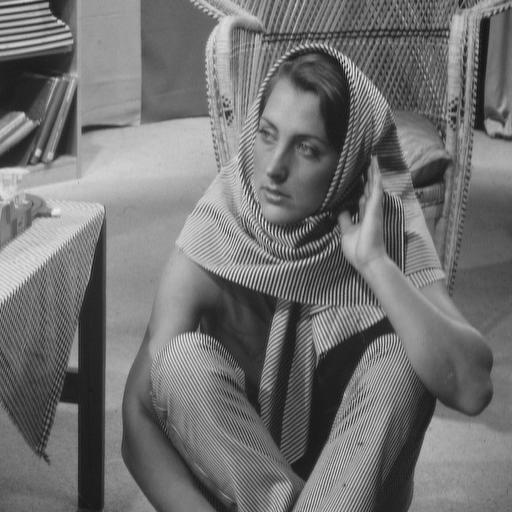
\includegraphics[width=.8\linewidth]{c1_1_1}}
\resizebox{5cm}{5cm}{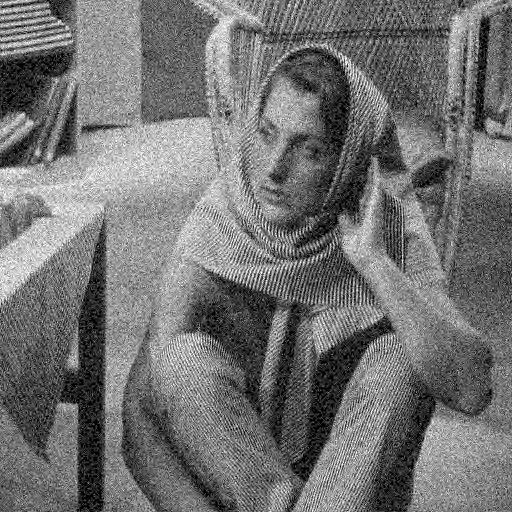
\includegraphics[width=.8\linewidth]{c1_2_1}}
\resizebox{5cm}{5cm}{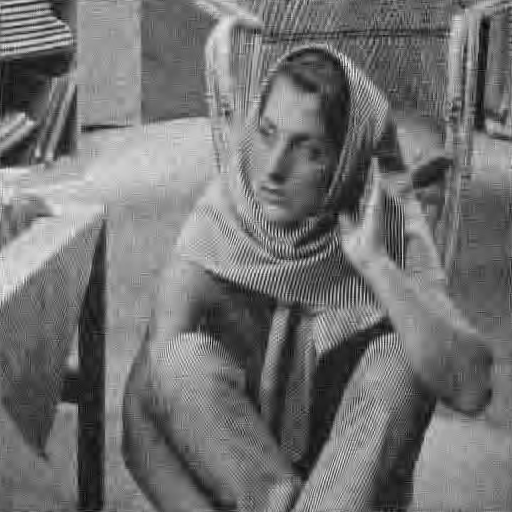
\includegraphics[width=.8\linewidth]{c1_3_1}}
\end{minipage}
\begin{minipage}[t]{0.5\textwidth}
\resizebox{5cm}{5cm}{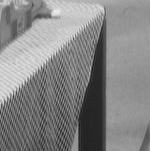
\includegraphics[width=1\linewidth]{c1_1_2}}
\resizebox{5cm}{5cm}{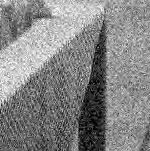
\includegraphics[width=1\linewidth]{c1_2_2}}
\resizebox{5cm}{5cm}{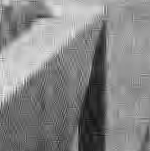
\includegraphics[width=1\linewidth]{c1_3_2}}
\end{minipage}
\caption{Denoising Result with $\sigma = 30$ for Barbara. Top: Original images and Zoom. Middle: `db2' Denoising. Bottom: `tf2' denoising.}
\end{figure}

%----------------------------------------------------------------------------------------
%	SECTION 2
%----------------------------------------------------------------------------------------

\section{Image Inpainting}
\subsection{PSNR results in image inpainting}
Inpainting process is more complicated than the denoising process in the way that recursive implementation is required for an effective inpainting process. Similar to the way we assessing the variables in denoising, several simple masks containing basic geometric graphs are selected and five filter banks are chosen in order to construct a comparision scheme. To further justify the choice of soft thresholding over hard thresholding in the process of inpainting, each test case is implemented for both thresholding methods. Similarly, the decomposition levels, initial threshold values and recursion times are selected form a range of feasible numbers for many times in order to reach the optimal result in extensive simulations.

\begin{figure}[H]
\begin{minipage}[t]{0.25\textwidth}
\resizebox{3.4cm}{3cm}{
\includegraphics[clip]{m_l_v}}\hspace{-0.4cm} 
\caption*{vertical line}
\resizebox{3.4cm}{3cm}{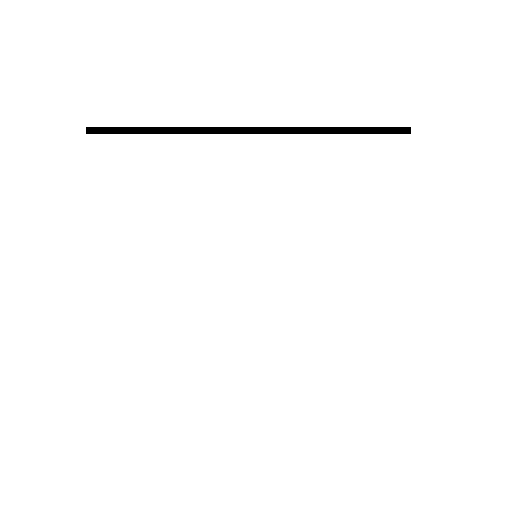
\includegraphics[clip]{m_l_h}}\hspace{-0.4cm} 
\caption*{horizontal line}
\end{minipage}\hspace{-0.2cm} 
\begin{minipage}[t]{0.25\textwidth}
\resizebox{3.4cm}{3cm}{
\includegraphics[clip]{m_l_rl}}\hspace{-0.4cm}
\caption*{right-left line}
\resizebox{3.4cm}{3cm}{
\includegraphics[clip]{m_l_lr}}\hspace{-0.4cm}
\caption*{left-right line}
\end{minipage}\hspace{-0.2cm} 
\begin{minipage}[t]{0.25\textwidth}
% \resizebox{6cm}{5cm}{\includegraphics{fig/p3/s_s2_1.eps}}\hfill
\resizebox{3.4cm}{3cm}{
\includegraphics[clip]{m_ring}}\hspace{-0.4cm}
\caption*{ring}
\resizebox{3.4cm}{3cm}{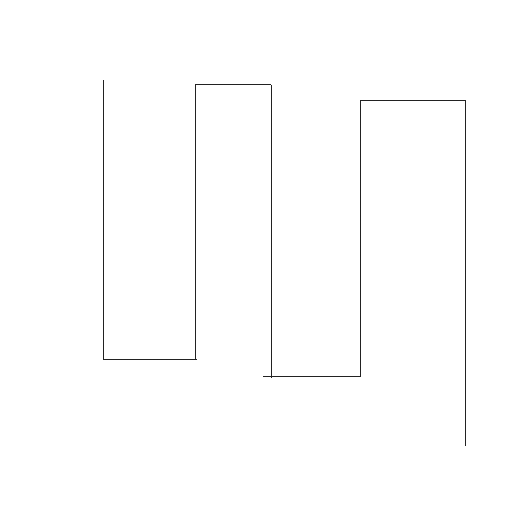
\includegraphics[clip]{m_line}}\hspace{-0.4cm}
\caption*{lines}
\end{minipage}\hspace{-0.2cm} 
\begin{minipage}[t]{0.25\textwidth}
\resizebox{3.4cm}{3cm}{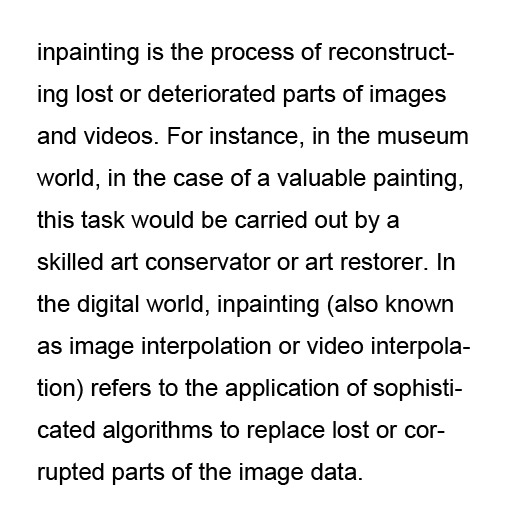
\includegraphics[clip]{m_text}}\hspace{-0.4cm}
\caption*{text}
\resizebox{3.4cm}{3cm}{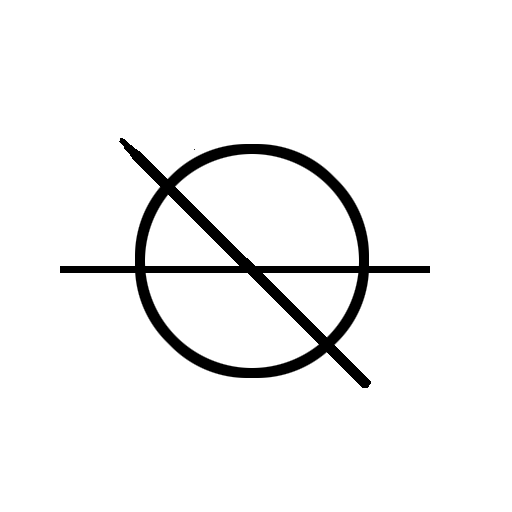
\includegraphics[clip]{m_combine}}
\caption*{combined mask}
\end{minipage}
\caption{Mask Figures}
\end{figure}

Figure 3.2 shows eight different masks used in our inpainting experiment including straight lines with four possible directions, a ring mask, text mask and a complicated mask combined of others. 


In the table 3.4, 3.5 and 3.6, the columns refer to fiver different filter banks, `db',`db2',`tf1',`tf2' and `tf3', the rows represent cases with different masks. And the second column named ``mask PSNR'' represent the corruption level of the mask image before the implementation of inpainting, surrounding values in the same row should be compared with the ``mask PSNR'' in order to justify the effectiveness of the corresponding method on the mask.\\

\begin{algorithm} 
\caption{Obtaining the optimum inpainting result}  
\label{alg:5}  
\begin{algorithmic}
\REQUIRE ~~\\ %算法的输入参数:Input  
A choices set L for possible levels (e.g. L= [3:7])
A choices set TV for possible threshold values (e.g. TV = [50:25:300])
A choices set R for possible recursion times (e.g. R =[3,5,7,9])
\ENSURE ~~\\ %算法的输出:Output  
The {opt}imum $PSNR_{opt}$ and the {opt}imum Indice $i_{opt},j_{opt}$
\STATE let $PSNR_{opt} = 0$
\STATE let $i_{opt} , j_{opt} =0, k_{opt} =0$
\FOR {i = 1: length(L)}
\STATE $l = L(i)$
\FOR {j = 1: length(TV)}
\STATE $th = TV(j)$
\FOR {k = 1: length(R)}
\STATE $rt = R(k)$
\STATE Using inpainting algorithm to compute the PSNR with Decomposition levels = l, threshold value = th, recursion time = rt
\IF {$PSNR > PSNR_{opt}$}
\STATE $PSNR_{opt} = PSNR, \; i_{opt} = i,\; j_{opt} = j, k_{opt} = k$ 
\ENDIF
\ENDFOR
\ENDFOR
\ENDFOR

\end{algorithmic}  
\end{algorithm}  

%Lena
% Please remember to add \use{multirow} to your document preamble in order to suppor multirow cells
\begin{table}[h]
\resizebox{1\textwidth}{!}{
\begin{tabular}{|l|l|l|l|l|l|l|l|l|l|l|l|}
\hline
\multicolumn{1}{|c}{\multirow{2}{*}{Lena}} & \multicolumn{1}{|c|}{\multirow{2}{*}{\begin{tabular}[c]{@{}c@{}}mask\\ PSNR\end{tabular}}} & \multicolumn{2}{|l}{db1}  & \multicolumn{2}{|l}{db2} & \multicolumn{2}{|l}{tf1} & \multicolumn{2}{|l}{tf2} & \multicolumn{2}{|l|}{tf3} \\ \cline{3-12} 
\multicolumn{1}{|c|}{} &  & hard & soft & hard & soft & hard & soft & hard & soft & hard & soft \\ \hline
vertical line   & 26.88 & 27.21 & 33.70 & 26.77 & 26.75 & 28.96 & 36.58 & 29.31 & 36.05 & 29.37 & \bf{36.62} \\ \hline
horizontal line & 24.39 & 24.65 & 32.43 & 25.03 & 24.98 & 25.81 & 37.00 & 25.91 & 39.16 & 26.51 & \bf{40.66} \\ \hline
right-left line & 23.01 & 25.75 & 32.03 & 23.32 & 23.29 & \bf{34.13} & 33.72 & 28.89 & 33.94 & 33.35 & 33.58 \\ \hline
left-right line & 24.62 & 27.92 & 32.99 & 24.98 & 24.87 & 38.41 & 37.82 & 33.03 & 37.37 & \bf{39.51} & 38.41 \\ \hline
ring            & 21.44 & 23.57 & 28.78 & 21.64 & 21.64 & 29.87 & 33.52 & 25.69 & 31.39 & 29.21 & \bf{33.72} \\ \hline
lines           & 27.18 & 28.51 & 43.32 & 33.69 & 32.64 & 32.74 & 43.36 & 37.23 & \bf{44.86} & 34.79 & 43.67 \\ \hline
text            & 15.75 & 26.52 & 30.95 & 16.08 & 16.13 & 33.75 & 33.13 & 33.71 & \bf{34.02} & 33.87 & 33.55 \\ \hline
combine         & 19.23 & 21.36 & 26.65 & 19.43 & 19.42 & 27.22 & \bf{31.39} & 24.16 & 30.50 & 27.00 & 31.25 \\ \hline
\end{tabular}}
\caption{Lena Inpainting}
\end{table}

%Boat
\begin{table}[h]
\resizebox{1\textwidth}{!}{
\begin{tabular}{|l|l|l|l|l|l|l|l|l|l|l|l|}
\hline
\multicolumn{1}{|c}{\multirow{2}{*}{Boat}} & \multicolumn{1}{|c|}{\multirow{2}{*}{\begin{tabular}[c]{@{}c@{}}mask\\ PSNR\end{tabular}}} & \multicolumn{2}{|l}{db1} & \multicolumn{2}{|l}{db2} & \multicolumn{2}{|l}{tf1} & \multicolumn{2}{|l}{tf2} & \multicolumn{2}{|l|}{tf3} \\ \cline{3-12} 
\multicolumn{1}{|c|}{} &  & hard & soft & hard & soft & hard & soft & hard & soft & hard & soft \\ \hline
vertical line   & 25.76 & 26.16 & 34.27 & 25.76 & 25.64 & 28.50 & 40.99 & 28.10 & 41.23 & 29.28 & \bf{41.28} \\ \hline
horizontal line & 24.96 & 25.22 & 33.91 & 25.60 & 25.55 & 26.44 & 39.68 & 26.35 & \bf{41.08} & 27.24 & 41.04 \\ \hline
right-left line & 23.39 & 26.26 & 31.67 & 23.66 & 23.63 & \bf{34.96} & 34.39 & 29.86 & 33.39 & 34.74 & 34.09 \\ \hline
left-right line & 23.39 & 26.29 & 33.45 & 23.73 & 23.67 & \bf{38.43} & 37.86 & 30.15 & 36.98 & 36.84 & 38.18 \\ \hline
ring            & 22.30 & 24.51 & 29.43 & 22.55 & 22.54 & 31.43 & 33.86 & 27.09 & 32.54 & 30.49 & \bf{34.16} \\ \hline
lines           & 27.28 & 28.73 & 42.03 & 32.67 & 32.15 & 33.87 & 41.59 & 37.06 & 43.01 & 35.75 & \bf{41.73} \\ \hline
text            & 15.39 & 26.73 & 30.39 & 15.72 & 15.73 & \bf{32.53} & 32.08 & 32.00 & 32.51 & 31.68 & 31.92 \\ \hline
combine         & 18.96 & 20.81 & 24.85 & 19.14 & 19.13 & 24.80 & \bf{29.38} & 22.79 & 28.50 & 24.90 & 29.26 \\ \hline
\end{tabular}}
\caption{Boat Inpainting}
\end{table}

%Barbara

\begin{table}[h]
\resizebox{1\textwidth}{!}{
\begin{tabular}{|l|l|l|l|l|l|l|l|l|l|l|l|}
\hline
\multicolumn{1}{|c}{\multirow{2}{*}{Barbara}} & \multicolumn{1}{|c|}{\multirow{2}{*}{\begin{tabular}[c]{@{}c@{}}mask\\ PSNR\end{tabular}}} & \multicolumn{2}{|l}{db1} & \multicolumn{2}{|l}{db2} & \multicolumn{2}{|l}{tf1} & \multicolumn{2}{|l}{tf2} & \multicolumn{2}{|l|}{tf3} \\ \cline{3-12} 
\multicolumn{1}{|c|}{} &  & hard & soft & hard & soft & hard & soft & hard & soft & hard & soft \\ \hline
vertical line   & 25.14 & 25.34 & 32.71 & 25.12 & 25.02 & 26.80 & \bf{45.54} & 26.44 & 42.06 & 27.06 & 43.35 \\ \hline
horizontal line & 25.49 & 25.79 & 31.95 & 26.13 & 26.07 & 26.76 & 36.31 & 27.31 & 36.39 & 27.53 & \bf{37.81} \\ \hline
right-left line & 24.37 & 27.62 & 33.38 & 24.63 & 24.60 & \bf{37.67} & 37.30 & 32.55 & 36.54 & 37.44 & 37.06 \\ \hline
left-right line & 22.92 & 25.66 & 32.37 & 23.22 & 23.17 & 36.19 & 35.97 & 29.52 & 35.79 & \bf{36.10} & 35.92 \\ \hline
ring            & 20.85 & 23.05 & 28.11 & 21.09 & 21.08 & 29.79 & 33.39 & 25.34 & 32.07 & 28.84 & \bf{33.70} \\ \hline
lines           & 27.53 & 29.18 & 40.95 & 31.12 & 31.92 & 34.52 & 40.84 & 39.67 & \bf{43.05} & 36.72 & 41.32 \\ \hline
text            & 16.31 & 26.98 & 30.03 & 16.54 & 16.59 & \bf{32.30} & 31.72 & 31.69 & 32.17 & 32.49 & 32.01 \\ \hline
combine         & 18.02 & 19.91 & 24.72 & 18.21 & 18.19 & 24.78 & 30.36 & 22.43 & 28.71 & 24.72 & 30.19 \\ \hline
\end{tabular}}
\caption{Barbara Inpainting}
\end{table}


\subsection{Performance analysis}
In terms of thresholding schemes,  the soft thresholding method shows a slight advantage in the process of image inpainting, whereas the hard thresholding also gets credit in some circumstances. As the optimal data highlighted in bold illustrates, the family of tight framelet filter banks demonstrated a great advantage in each test case. Figure 3.3 shows the comparison of inpainting results with text mask using orthogonal filter bank Haar and the tight framelet filter bank `tf1' correspondingly, and the second column shows the zoom in details. As we see, tight framelet filter bank is an effective tool since it has the property of redundancy and Figure 3.3 also indicates redundancy is desirable in some applications such as image inpainting. 
\begin{figure}[H]
\begin{minipage}[t]{0.5\textwidth}
\centering
\resizebox{5cm}{5cm}{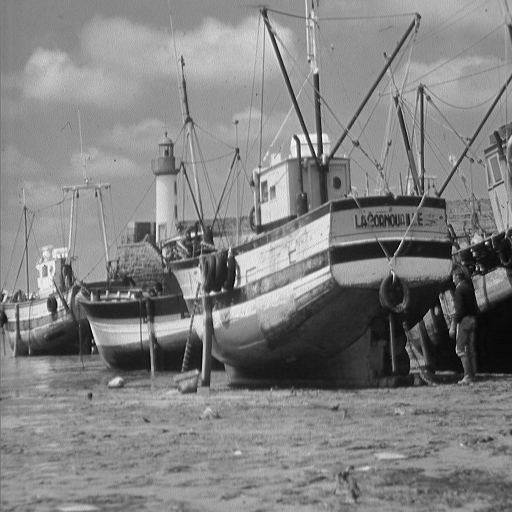
\includegraphics[width=.8\linewidth]{c2_1_1}}
\resizebox{5cm}{5cm}{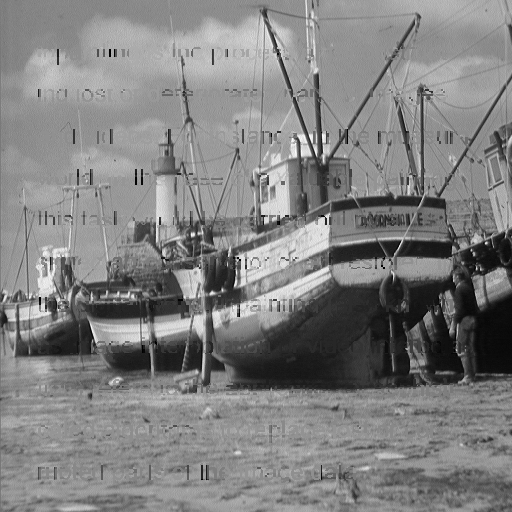
\includegraphics[width=.8\linewidth]{c2_2_1}}
\resizebox{5cm}{5cm}{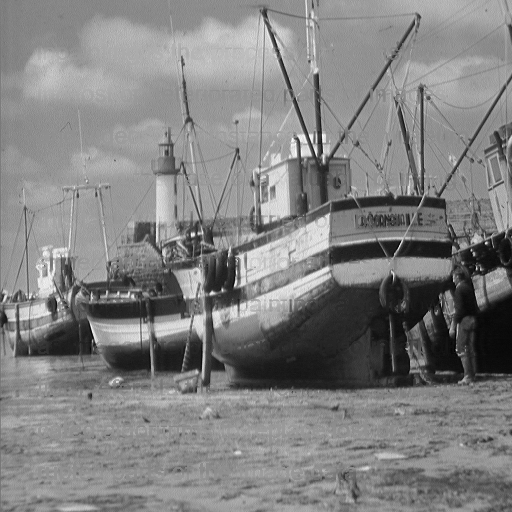
\includegraphics[width=.8\linewidth]{c2_3_1}}
\end{minipage}
\begin{minipage}[t]{0.5\textwidth}
\resizebox{5cm}{5cm}{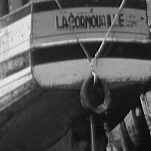
\includegraphics[width=1\linewidth]{c2_1_2}}
\resizebox{5cm}{5cm}{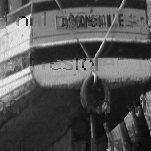
\includegraphics[width=1\linewidth]{c2_2_2}}
\resizebox{5cm}{5cm}{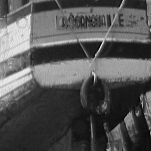
\includegraphics[width=1\linewidth]{c2_3_2}}
\end{minipage}
\caption{Inpainting Result with `text' mask for Boat. Top: Original images and Zoom. Middle: `db1' Inpainting. Bottom: `tf1' inpainting.}
\end{figure}
